\header{
    \headtitle{A la claire fontaine} \label{a-la-claire-fontaine}
    %
    %Chant ancien publié en 1704
    \insertComment{}{}
}

\enluminure{4}{\href{https://www.youtube.com/watch?v=-VctOj6Bm4Y}{A}}{la claire} fontaine,
\\Hier après dîner,
\\Y avait trois capitaines
\\Qui m'ont déshabillée.
\dualcol{
\textbf{Refrain :}
\\Il y a longtemps que je baise
\\Jamais je ne m'arrêterai
\\\\Et là sous la verdure,
\\Tous les trois à la fois,
\\M'ont glissé leur nature
\\Dans tous les bons endroits.
\\\\Après les capitaines,
\\Vint le gentil meunier,
\\M'a pris la turlutaine
\\Et s'en est régalé.
\\\\Puis ce fut le notaire,
\\Passant sur le chemin,
\\Qui me mit son affaire
\\Gentiment dans la main.
\\\\Après quoi les gendarmes,
\\Vinrent, les polissons,
\\Tous deux verser leurs larmes
\\Sur mon petit gazon.
\\\\Là je vis sous la lune,
\\Arriver le bedeau,
\\Qui me dit: " Viens, ma brune,
\\Faire la bête à deux dos! "
\\\\Puis le maître d'école,
\\A son tour est venu,
\\M'a glissé son obole
\\Dans l'abricot fendu.
\\\\Enfin tout le village,
\\Par l'amour alléché,
\\Me fit un ramonage
\\Dont je me souviendrai.
\\\\Quelle belle nuit pour une femme,
\\Quel voluptueux gala,
\\Car comme vous mesdames,
\\Je ne pense qu'à ça.
\\
}
\begin{center}
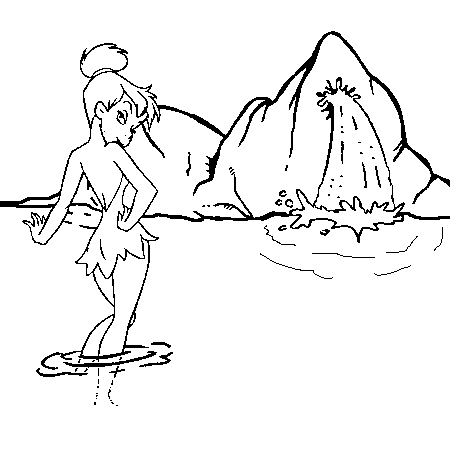
\includegraphics[width=0.35\textwidth]{images/a-la-claire-fontaine.png}
\end{center}

\breakpage